\documentclass[12pt, letterpaper, twoside]{article}
\usepackage[utf8]{inputenc}
\usepackage[spanish]{babel}
\usepackage{amsmath, amsfonts, amssymb, amsthm}
\usepackage[left = 2cm, right = 2cm, top = 2cm, bottom = 2cm]{geometry}

\title{Grafos}

%Estilo de la página
\usepackage{fancybox, fancyhdr}
\pagestyle{fancy}
\fancyhf{}
\fancyhead[LE,RO]{\small{\leftmark}}
\fancyfoot[CE,CO]{\thepage}
\renewcommand{\headrulewidth}{2 pt}

%Imagenes
\usepackage{graphicx}
\graphicspath{{Imagenes/}}

%Estilo del codigo
\usepackage{listings}
\usepackage[dvipsnames]{xcolor}
\lstset{  
	language         = C++, 
	xleftmargin      = 1 cm,
	numbers          = left,
	numberstyle      = \tiny\textbf,	
	basicstyle       = \footnotesize,
	keywordstyle     = \color{blue},
	directivestyle   = \color{Green},
	commentstyle     = \color{purple},
	stringstyle      = \color{blue},
	showstringspaces = false,
	breaklines       = true,
}

%Documento
\begin{document}

\section{Caminos más cortos.}

Consideremos un grafo $G = (V, E)$ donde cada arista $(u, v)$ tiene una longitud $d(u,v) > 0$. El camino más corto entre dos vértices es aquel que minimiza la longitud total del camino.

\subsection{Algoritmo de Dijkstra}

Complejidad: $O((|E| + |V|) \log|V|)$.

\lstinputlisting[firstline = 6]{Dijkstra.cpp} \medskip

\begin{tabular}{|p{7cm}|p{7cm}|}
\hline
\textbf{Entrada} & \textbf{Salida}\\ \hline
6 7    & 0: -1 0\\
0 1 4  & 1: 0 4\\
1 3 10 & 2: 0 2\\
3 5 11 & 3: 4 9\\
1 2 5  & 4: 2 5\\
2 0 2  & 5: 3 20\\
2 4 3  & \\
4 3 4  & \\
0      & \\ \hline
\end{tabular}

\begin{figure}[h]
\centering
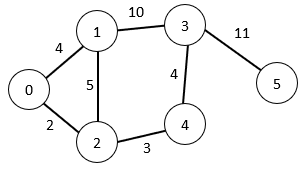
\includegraphics[width = 0.45\textwidth]{ShortestPath.png}

\caption{Ejemplo.}
\end{figure}

\newpage

\section{Árbol de expansión mínima.}

Consideremos un grafo $G = (V, E)$ donde cada arista $(u, v)$ tiene un peso $w(u,v)$. Un árbol de expansión mínima es un subgrafo de $G$ que es árbol y minimiza la suma de los pesos.

\subsection{Algoritmo de Kruskal}

Complejidad: $O(|E| \log|V|)$.

\lstinputlisting[firstline = 6]{Kruskal.cpp} \medskip

\begin{tabular}{|p{7cm}|p{7cm}|}
\hline
\textbf{Entrada} & \textbf{Salida}\\ \hline
6 8    & Peso total: 18\\
0 1 2  & 0 3 1\\
0 3 1  & 3 5 1\\
3 1 9  & 0 1 2\\
4 1 10 & 3 4 3\\
3 4 3  & 2 0 11\\
2 0 11 & \\
2 5 20 & \\
3 5 1  & \\ \hline
\end{tabular}

\begin{figure}[h]
\centering
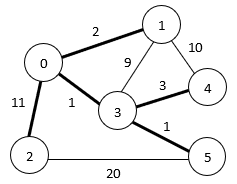
\includegraphics[width = 0.35\textwidth]{MST.png}

\caption{Ejemplo.}
\end{figure}

\newpage

\section{Orden topológico.}

Consideremos un grafo dirigido acíclico $G = (V, E)$. Un orden topológico es un ordenamiento lineal de los vértices en donde las aristas conectan solamente con vértices posteriores.

\subsection{Algoritmo}

Complejidad: $O(|V| + |E|)$.

\lstinputlisting[firstline = 6]{TopoSort.cpp} \medskip

\begin{tabular}{|p{7cm}|p{7cm}|}
\hline
\textbf{Entrada} & \textbf{Salida}\\ \hline
7 9 & 6 0 1 2 5 4 3\\
6 1 & \\
6 5 & \\
0 1 & \\
1 5 & \\
0 2 & \\
1 2 & \\
2 3 & \\
5 3 & \\ 
5 4 & \\ \hline
\end{tabular}

\begin{figure}[h]
	\centering
	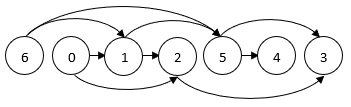
\includegraphics[width = 0.6\textwidth]{TopoSort.png}
	
	\caption{Ejemplo.}
\end{figure}

\newpage

\section{Máximo flujo.}

Consideremos un grafo dirigido $G = (V, E)$ donde cada arista $(u, v)$ tiene asociada una capacidad $c(u,v) > 0$. Un flujo de $s$ a $t$ es una función que a cada arista le asigna un número $f(u,v)$ que satisface
\begin{itemize}
\item $f(u, v) \leq c(u,v)$.
\item Para cualquier vértice $v \neq s, t$, el flujo que entra es igual al flujo que sale; $s$ solo tiene flujo saliente y $t$ solo tiene flujo entrante.
\end{itemize}
El flujo total es el flujo que sale de $s$.

\subsection{Algoritmo de Edmonds-Karp}

Complejidad: $O(|V||E|^2)$.

\lstinputlisting[firstline = 6]{Edmonds-Karp.cpp} \medskip

\begin{tabular}{|p{7cm}|p{7cm}|}
\hline
\textbf{Entrada} & \textbf{Salida}\\ \hline
6 8 & Flujo maximo: 23\\
0 1 11 & 0 1: 11/11\\
0 2 12 & 0 2: 12/12\\
1 3 12 & 1 3: 12/12\\
2 1 1  & 2 1: 1/1\\
2 4 11 & 2 4: 11/11\\
4 3 7  & 3 5: 18/19\\
3 5 19 & 4 3: 6/7\\
4 5 5 & 4 5: 5/5\\ 
0 5 & \\ \hline
\end{tabular}

\begin{figure}[h]
\centering
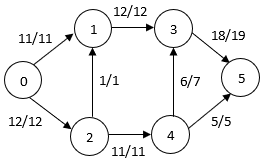
\includegraphics[width = 0.45\textwidth]{MaxFlow.png}

\caption{Ejemplo.}
\end{figure}

\newpage

\section{Emparejamiento máximo.}

Consideremos un grafo bipartito $G = (U \cup V, E)$. Un emparejamiento de $G$ es un subgrafo en donde cada vértice pertenece a lo más a una arista.

\subsection{Algoritmo de Hopcroft-Karp}

Complejidad: $O(|E|\sqrt{|V|})$.

\lstinputlisting[firstline = 7]{Hopcroft-Karp.cpp} \medskip

\begin{tabular}{|p{7cm}|p{7cm}|}
\hline
\textbf{Entrada} & \textbf{Salida}\\ \hline
5 4 8 & Emparejamiento: 3\\
1 1   & 1 - 1\\
2 1   & 2 - 3\\
2 3   & 3 - 2\\
3 2   & \\
3 3   & \\
3 4   & \\
4 3   & \\
5 3   & \\ \hline
\end{tabular}

\begin{figure}[ht]
\centering
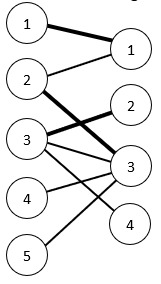
\includegraphics[height = 0.3\textheight]{MaxMatching.png}	

\caption{Ejemplo.}
\end{figure}

\newpage

\end{document}